\chapter{Introduction}
\label{chap:introduction}

\section{Data structure centric distributed systems}

\TODO{How do I write something general about data locality and load imbalance?}
The use of in-memory data processing systems has recently grown as a result of
different advances in computer hardware. Lower operating cost of DRAM means we
are incentivized to design systems that sacrifice memory usage for performance.
Faster network interconnects reduce the latency of communication between
machines, minimizing the performance cost of scaling out server software.
Analogically similar to the above, persistent memory tightens the performance
gap between in-memory data processing and file system persistence layer,
allowing applications to persist data structures as fast as they can use them
in main memory, as they are kept consistent across operations.

\TODO{citations?}
these improvements have collectively and independently cast doubt on the precondition of
``slow devices, fast CPU'' by gradually shifting both latency and throughput
bottlenecks towards the classical position of the processor and the kernel.
This had encouraged research towards building systems which manage their
network communication and storage more closely. User space networking \TODO{ cite
DPDK and/or the likes and things that use them? what else?} and managing high
traffic data structures like hash-tables and balanced binary search trees
\TODO{mention masstree or similar, and some usages?} in the application are
both research trends in developing what we call \emph{data structure centric}
applications \TODO{citations/examples?}. Indeed the operating system kernel provides networking and high
level interface to useful data structures (e.g. through the interface of file
systems) but for high performance applications, the performance gain from using
a specialized way of managing data is worth the complexity.
Some of these systems target low latency, but all of them have to provide
a solution for higher throughput workloads. As we exhaust the resource limits
of a single machine, this becomes synonymous to how the system scales out to
multiple machines.\TODO{suitable point to break the paragraph?}

In multi-machine environments, any non-trivial (read-only in essence) system
faces problems that also become apparent when we cross the single-threaded
to multi-threaded boundary: how to manage accesses to shared data and where to
schedule computations. These in part translate to two separate objectives in
the design of data structure centric distributed systems. \TODO{should I use a
hyphen in there?} \TODO{is centric a word?}
\begin{itemize}
    \item How to keep computation close to the data that it uses (Locality)
    \item Where to process each request to avoid overloading any of the machines (Load balancing)
\end{itemize}





\section{Locality and load balancing}
System designers have came up with various solutions to to keep their
computations as close as possible to their data.

Some applications can tolerate relaxed guarantees for how reads and writes are
executed. \TODO{mention a few examples and their requirements?}
Typically replicas are or can be used in these applications as they can be
used to process certain (particularly read-only) requests based on the
consistency requirements of the system.

Not paying attention to the locality constraints and remote access penalties
and simply contending for resources results (e.g. optimistic concurrency
control) will result in poor performance in workloads with highly contended
accesses.

\begin{figure}[hbt!]


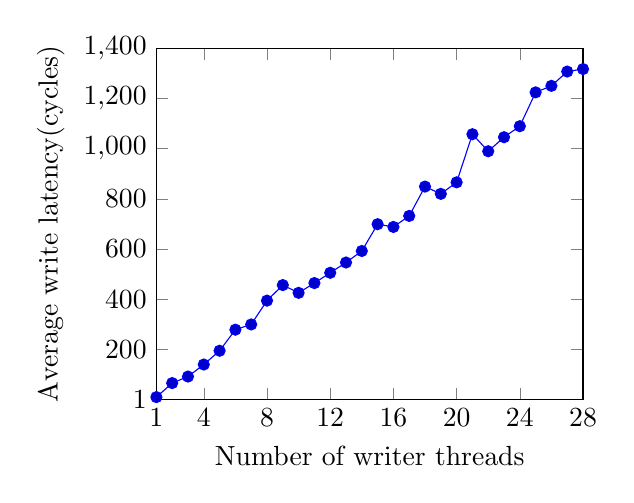
\begin{tikzpicture}[baseline]
\begin{axis}[
width=7cm,
xmin=1,xmax=28,
ymin= 0,ymax=1400,
xlabel=Number of writer threads,ylabel=Average write latency(cycles),
xtick={1,4,8,...,28},
ytick={1,200,400,...,1400},
]
\addplot coordinates{
  (1,9) (2,65) (3,91) (4,139) (5,194) (6,278) (7,299) (8,394) (9,456) (10,425)
  (11,464) (12,505) (13,546) (14,592) (15,699) (16,688) (17,732) (18,849)
  (19,820) (20,866) (21,1058) (22,990) (23,1046) (24,1090) (25,1225) (26,1251)
  (27,1308) (28,1318)
};
\end{axis}
\end{tikzpicture}%
~%
%
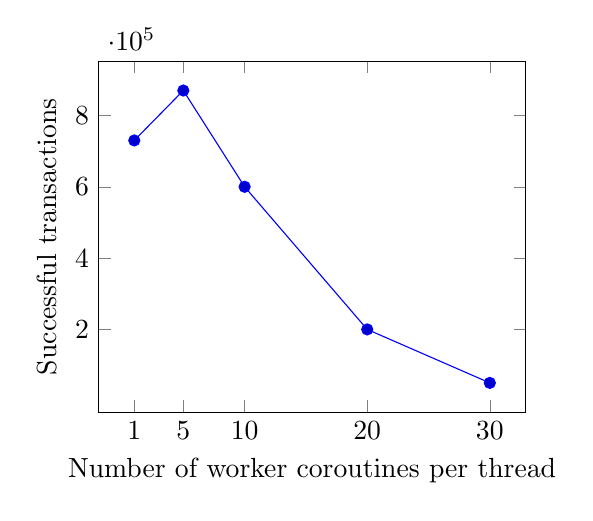
\begin{tikzpicture}[baseline]
\begin{axis}[
width=7cm,
% xmin=0,xmax=32,
% ymin= 0,ymax=0.10,
xlabel=Number of worker coroutines per thread,ylabel=Successful transactions,
xtick={1,5,10,20,30},
ytick={200000,400000,600000,800000,1000000},
]
\addplot coordinates{
    (1,730000) (5,870000) (10,600000) (20,200000) (30,50000)
};
\end{axis}
\end{tikzpicture}%

\caption{
    The left figure, similar to one from \cite{boyd2014oplog}, shows how
    performance degrades as different cores contend on a lock for synchronized
    write access to a shared byte. To remedy this, they propose a batching
    technique. The right figure shows how increasing
    the number of coroutines in a distributed transaction processing system
    \cite{kalia2016fasst} impacts performance on a contended workload.
      }
\label{fig:contention_penalty}

\end{figure}

Sharding techniques are also used extensively, allowing system designers to
choose almost any point in the spectrum of design space between high-locality;
coarser load balancing (e.g. partitioning user data by user id) and
low-locality; better load balancing (e.g. random sharding).

An important property of some of these designs is modularity, as
a result of the problem space being composable, with similarities to how the
memory
hierarchy is laid out and how similar problems arise at every level. For
example all of the above remain
relevant even after one ``layer'' of randomly sharding the data or the requests,
as the designer of the system is yet to decide what is the consistency
requirements of the system within and in between the shards, as well as
enjoying the freedom of applying other techniques in the higher layers.
This suggests that
it would make sense for the solutions targeting locality and
load balancing to attend to a particular horizontal slice of the problem,
limiting the conditions and requirements. For example a high performance
locking scheme can choose to provide the flexibility to be incorporated in a
sharding scheme to manage cross-partition accesses, as opposed to being bound
be used in a specific partitioning scenario.
Not only this guideline
will make the design of systems simpler and more effective, it allows us to
fuse independent solutions for different locality and load balancing
sub-problems when designing a system.

With that in mind, we have limited our target domain to the ``layer'' where each
subset of read and write requests can be encapsulated with the data structures
that they need to access, creating a scheduling unit which along with its
respective computation, will be placed on a single machine. The way the
application organizes its workload into these units (upper design layers)
and what the system decides to do inside each one of these units (lower design
layers), as well as how these units communicate, will be left to the
application, which will be responsible for all the plumbing, with the gained
benefit of composability of different solutions.


\TODO{Is this section full of useless jargon? Are there too quick shifts from general hand waving
to specific details? Does it get a message through? Do we need to change the
section title? Would a figure be useful?}

\newpage



\section{Migrating data structures}






\section{RDMA background}






\section{Contributions}
We propose the design and an implementation of slope





\section{Outline}

